\section{Systemüberblick und verteilte Kommunikation}

Das ReSiLENT-System gliedert sich in zwei logische Domänen: die
\textbf{Charging Station} mit dem eingebetteten Detection-Client sowie
das \textbf{Cloud Dashboard} zur zentralen Visualisierung und Auswertung.
Beide Domänen sind über ein privates Peer-to-Peer-Netzwerk auf Basis des
\textit{InterPlanetary File System} (IPFS) lose gekoppelt. Anstelle direkter
IP-zu-IP-Verbindungen erfolgt der Datenaustausch über inhaltsadressierte
Bezeichner (\textit{Content Identifier}, CIDs), wodurch keine einzelne
Ausfallstelle existiert und die Kommunikation robust gegenüber
netzwerktopologischen Veränderungen ist.

\begin{figure}[h]
    \centering
    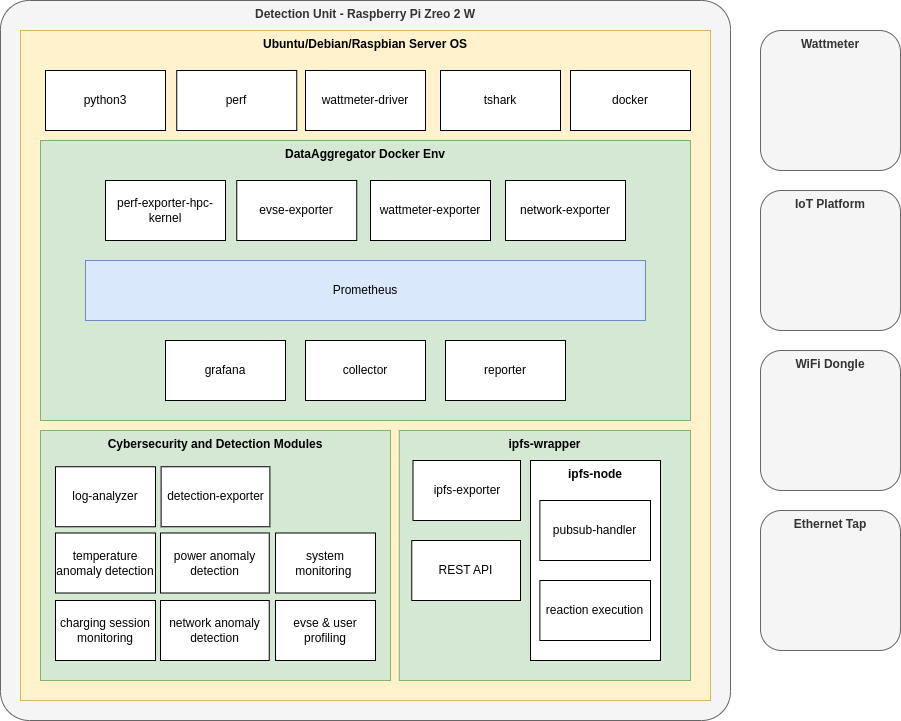
\includegraphics[width=\textwidth]{./figures/deployment_software_modules_v1.drawio.png}
    \caption{Gesamtarchitektur des ReSiLENT-Systems mit Charging Station
    und Cloud Dashboard}
    \label{fig:system_overview}
\end{figure}

Abbildung~\ref{fig:system_overview} zeigt die Gesamtarchitektur des Systems
mit Fokus auf die in jeder Wallbox eingebettete Detection Unit, die auf einem
Raspberry Pi Zero 2~W unter einem Ubuntu-Raspbian-Server-Betriebssystem
betrieben wird. Als zentrales Laufzeitmodul fungiert der \textit{Data
Aggregator}, der die erfassten Sensordaten der Wallbox über Prometheus
bereitstellt und sowohl den Cybersecurity- und Detection-Modulen als auch
Werkzeugen zur Datenaufbereitung zugänglich macht.

Die Architektur ist auf kollaborative Angriffserkennung ausgelegt: Über den
\textit{ipfs-wrapper} und dessen \textbf{Publish-Subscribe-Mechanismus} (detailliert in Abbildung~\ref{fig:ipfs_network}) teilen Ladesäulen sicherheitsrelevante
Kontextinformationen mit allen Netzwerkteilnehmern und erhöhen so die
situative Wahrnehmung (\textit{Situational Awareness}) über die gesamte
Ladeinfrastruktur hinweg.

\subsection{Privates IPFS-Netzwerk und Peer-to-Peer-Datenaustausch}

Für die verteilte Kommunikation zwischen den Detection Units und dem Cloud
Dashboard wird ein \textbf{privates IPFS-Netzwerk} eingesetzt. Im Gegensatz
zum öffentlichen IPFS-Netz wird der Zugang durch einen gemeinsamen
\textit{Swarm Key} beschränkt, sodass ausschließlich autorisierte Knoten dem
Netzwerk beitreten können. Die Netzwerktopologie ist in
Abbildung~\ref{fig:ipfs_network} dargestellt.

\begin{figure}[h]
    \centering
    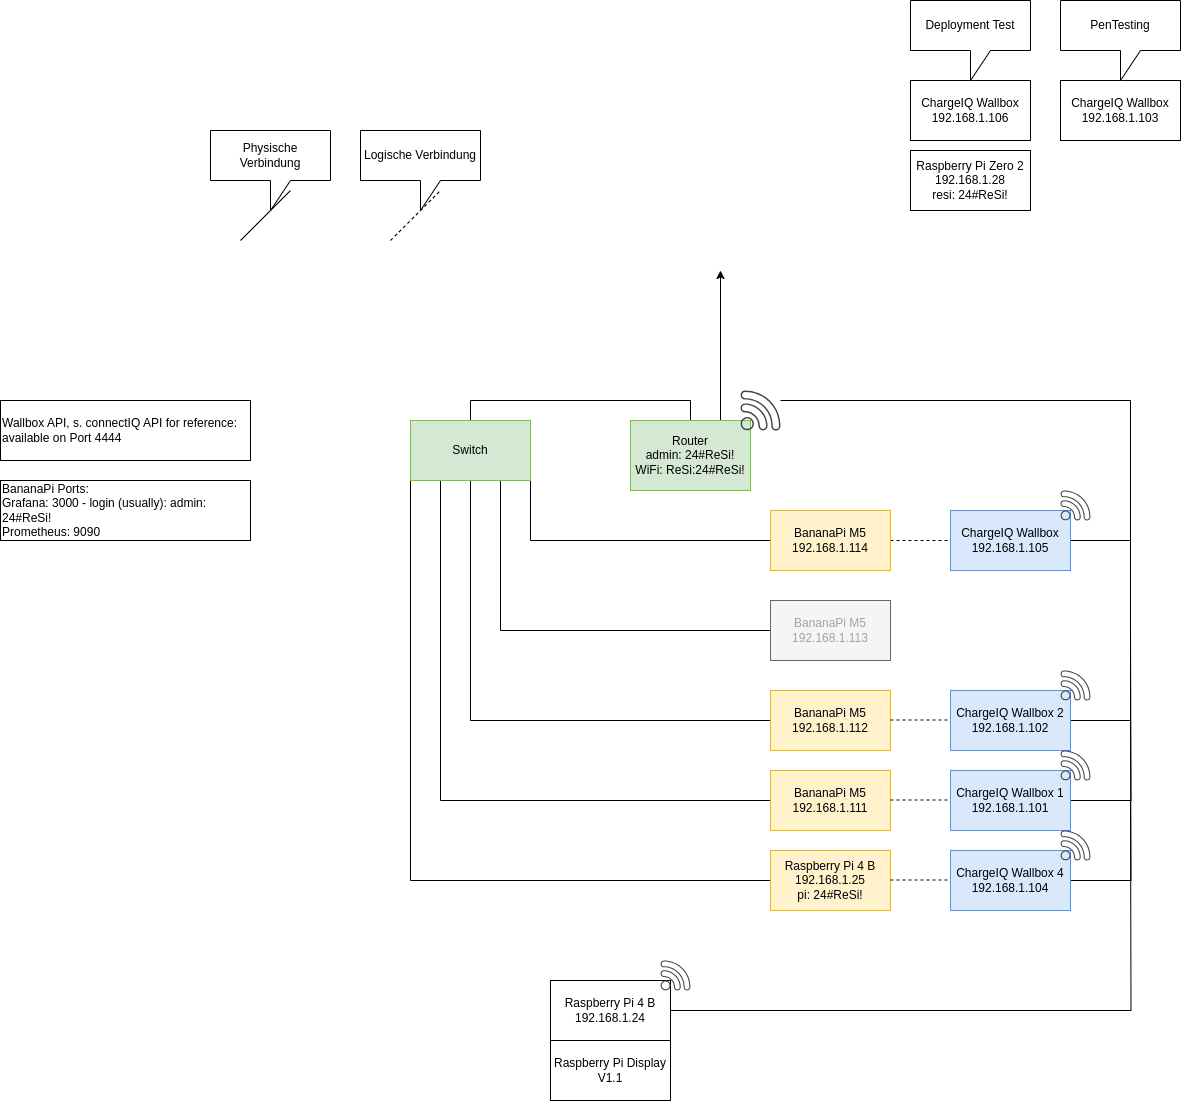
\includegraphics[width=0.75\textwidth]{./figures/SystemDiagramv2.drawio.png}
    \caption{Topologie des privaten IPFS-Netzwerks mit Bootstrap-Node und
    Client-Peers}
    \label{fig:ipfs_network}
\end{figure}

Der Netzbeitritt erfolgt über einen dedizierten \textbf{Bootstrap-Node},
der auf dem Server des Cloud Dashboards betrieben wird. Neue Peers melden
sich beim Bootstrap-Node an, erhalten die Multiaddresses (\textit{MADDR})
der bekannten Peers und kommunizieren anschließend direkt miteinander, ohne
den Bootstrap-Node als Relay zu verwenden. Jede Detection Unit betreibt
einen lokalen \textbf{IPFS-Peer-Daemon}, der über den \texttt{ipfs-wrapper}
-- wie in Abbildung~\ref{fig:dataflow} dargestellt -- in die
Systemarchitektur eingebunden ist.

Für die Benachrichtigung über neue Daten wird der
\textbf{Publish-Subscribe-Mechanismus} von IPFS genutzt: Sobald eine
Detection Unit neue Messdaten veröffentlicht, sendet sie die zugehörige CID
zusammen mit der eigenen MADDR über einen gemeinsam abonnierten Kanal an
alle Teilnehmer. Die Empfänger rufen die Datei daraufhin direkt beim
Ursprungs-Peer ab. Da eine CID dem kryptografischen Hash des jeweiligen
Inhalts entspricht, ist die Datenintegrität implizit gewährleistet, ohne
dass zusätzliche Signaturmechanismen erforderlich sind.

\subsection{End-to-End-Datenfluss}

Der vollständige Datenfluss vom Sensor bis zur Visualisierung lässt sich in drei Phasen unterteilen: Datenerhebung und Aggregation auf der Charging Station, Transport über das IPFS-Netz sowie Persistierung und Darstellung im Cloud Dashboard. Das Sequenzdiagramm in Abbildung~\ref{fig:sequence} sowie der Datenfluss in Abbildung~\ref{fig:dataflow} illustrieren diesen Ablauf.

\begin{figure}[h]
    \centering
    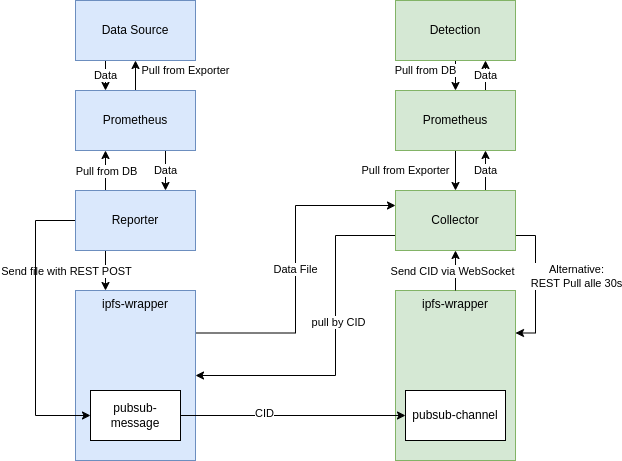
\includegraphics[width=\textwidth]{./figures/DataFlowIPFS.drawio.png}
    \caption{Datenfluss zwischen Charging Station (blau) und Cloud Dashboard (grün) über IPFS}
    \label{fig:dataflow}
\end{figure}

\begin{figure}[h]
    \centering
    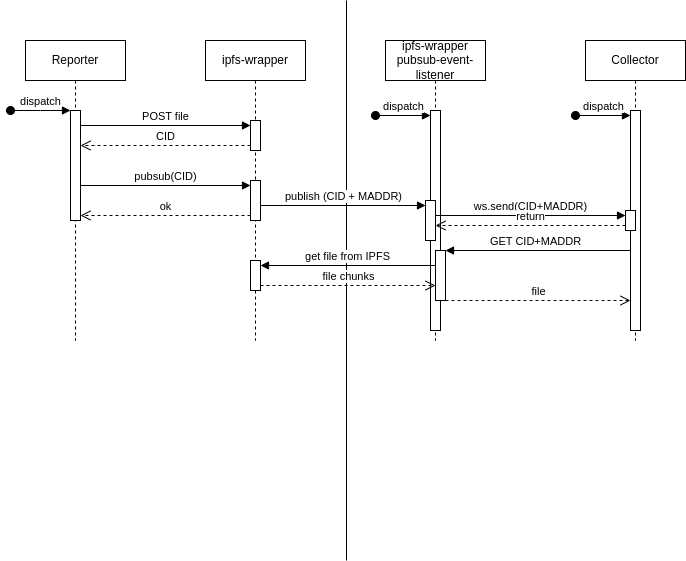
\includegraphics[width=0.85\textwidth]{./figures/Sequenzdiagramm_Datenfluss.drawio.png}
    \caption{Sequenzdiagramm des IPFS-basierten Datenaustausches}
    \label{fig:sequence}
\end{figure}

\paragraph{Datenerhebung (Charging Station)}
Der \textit{Aggregator} innerhalb des Detection-Clients sammelt Messdaten aus drei Quellen: EVSE-spezifische Daten werden über die \textit{Lokale API} des IoT-Moduls bezogen, Systemmetriken des Hosts über einen \textit{Node Exporter}, sowie interne Detektionsergebnisse über interne Komponenten. Prometheus scraped alle Exporter in konfigurierbaren Intervallen. Der \textit{Reporter} liest die aggregierten Daten aus der Prometheus-Datenbank und übermittelt sie per \textbf{HTTP POST} an den \texttt{ipfs-wrapper}.

\paragraph{Transport (IPFS-Netzwerk)}
Der \texttt{ipfs-wrapper} nimmt die Datei entgegen, publiziert sie im lokalen IPFS-Node und erhält eine CID zurück. Anschließend wird die CID zusammen mit der eigenen MADDR über den konfigurierten \textbf{Publish-Subscribe-Mechanismus} im privaten IPFS-Netz verbreitet. Die eigentlichen Messdaten werden dabei nicht aktiv gepusht, lediglich der Zeiger (CID) wird distribuiert.

\paragraph{Persistierung und Visualisierung (Cloud Dashboard)}
Auf der Serverseite empfängt der \textit{Publish-Subscribe-Event-Listener} des \texttt{ipfs-wrapper} die CID und MADDR und leitet diese per \textbf{WebSocket} an den \textit{Collector} weiter. Der Collector fordert daraufhin die vollständige Datei über den lokalen IPFS-Peer an, der sie in Chunks vom Ursprungs-Peer abruft. Der \textit{File Extractor} verarbeitet die Rohdaten und persistiert die Messwerte in \textbf{InfluxDB}. Grafana greift auf InfluxDB zu und stellt die Zeitreihendaten im Dashboard dar (vgl. Abbildung~\ref{fig:cloud_dashboard}).

\begin{figure}[H]
    \centering
    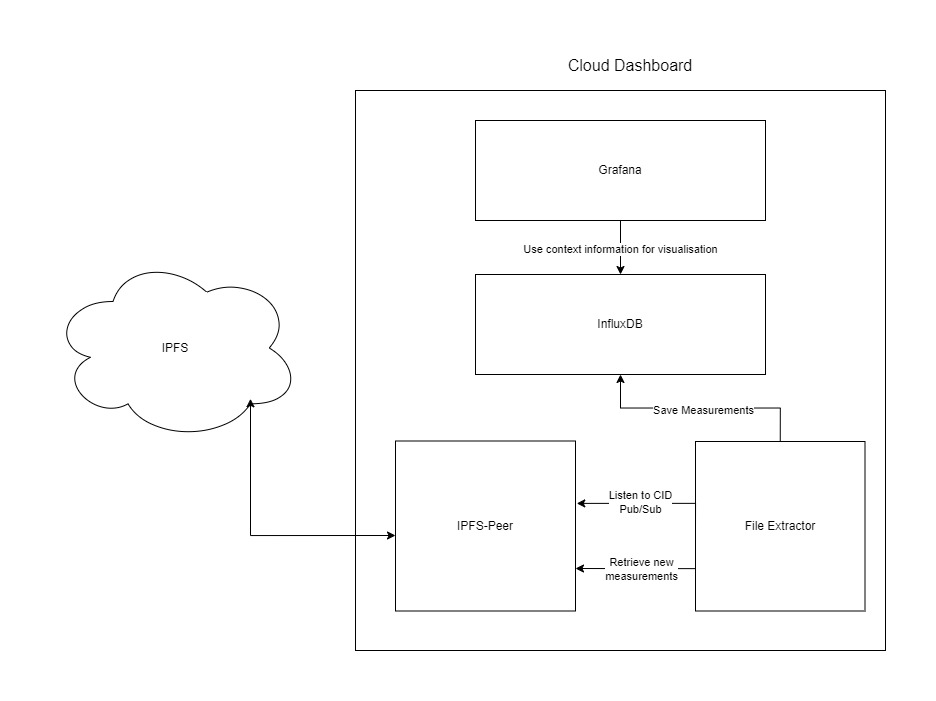
\includegraphics[width=0.75\textwidth]{./figures/Cloud-Dashboard.jpg}
    \caption{Komponenten des Cloud Dashboards: IPFS-Peer, File Extractor, InfluxDB und Grafana}
    \label{fig:cloud_dashboard}
\end{figure}